%%% A template for Acta Philosophica Gothoburgensia.
%%% For use with XeLaTeX and KOMA-Script.
%%% Version 2021 (April)
\documentclass[fontsize=14pt,
               paper=297mm:210mm,
               twoside,
               pagesize=pdftex,
               DIV=calc
]{scrbook}

\newif\ifdraft
%%% The following line sets a number of draft-related options. Remove it once you're done writing.
\drafttrue

%%% Must be placed after \ifdraft (and \drafttrue, if used)
\usepackage{ACTA}

%%% Only used for placeholder text.
\usepackage{lipsum}

%%% MACROS
%%%
%%% Give the title of the book here
\title{The name of the book}
%%% Give the subtitle here
\subtitle{Then the subtitle of the book}
%%% Give the author name here
\author{Thesis author}
%%% Set the series number here.
\titlehead{Acta Philosophica Gothoburgensia XX}
%%% Give the ISBN for the printed version here.
\isbnp{978-91-7346-xxx-x}
%%% Give the ISBN for the digital (pdf) version here.
\isbnd{978-91-7346-xxy-y}


%%% NOTE: By default, the even-page header is set to be the title of the book.
%%% If your title is very long, or otherwise unsuitable to put in the header,
%%% you can manually set the running header below. Use lowercase - it is turned
%%% into small caps (as required) automatically.
%
%\runningheader{short header}


%%% For bibliography formatting according to ACTA regulations. If you don't want to use
%%% natbib, you'll have to make the two tweaks below in some other (to me unknown) way.
\usepackage{natbib}
\bibliographystyle{apalike} % or whatever you prefer
\setlength{\bibhang}{0.6cm}
\setlength{\bibsep}{6pt}

 
%%% Here's the document.
%%%
%%%
 
 
\begin{document}
%%% For hyphenation, etc. Can be changed to USenglish, if preferred.
\selectlanguage{UKenglish}

\frontmatter
\pagestyle{empty}
%%% These two lines includes the files typesetting the title pages and various frontmatter.
%%% Make sure to edit these files to insert the correct information.
%%% ACTA-titlepages.tex

%%% Failsafe
\fontsize{14}{18}\selectfont
%%% Half-title page/smutstitelsida
% 
%%% Title is supposed to start 120pt (= 42mm) below start of type area. 
%%% In reality, the Word template puts it 44mm below start of the type area. Baseline at 49mm.
%%% A vspace of 31.5mm accomplishes this... (almost equal to 42mm minus a baselineskip of 28pt)
\vspace*{31.5mm}
\begin{center}
\fontsize{22}{28}\selectfont %calculated line spacing
 \makeatletter{\@title\par}\makeatother
\end{center}

\cleardoublepage

%%% Title page
\newgeometry{top=13mm,bottom=18.5mm,left=30mm,right=30mm} %RB: all positions depend on these top and bottom margins!

\begin{center}
\usekomafont{titlehead}\selectfont
\makeatletter{\MakeLowercase{acta universitatis gothoburgensis\\\@titlehead}\par}\makeatother
\end{center}
\vspace*{38.7mm} % tweaked after optical inspection
\begin{addmargin}{0.63cm}
\begin{flushleft}

\makeatletter\ifx\@subtitle\@empty\makeatother
\usekomafont{title}\selectfont
\makeatletter{\@title\par}\makeatother 
\par \vspace{\baselineskip}
\usekomafont{author}\selectfont
\makeatletter{\@author\par}\makeatother

\else
\usekomafont{title}\selectfont
\makeatletter{\@title\par}\makeatother % \par \vspace{\baselineskip}

\vspace{12pt}
\usekomafont{subtitle}\selectfont
\makeatletter{\@subtitle\par}\makeatother
\usekomafont{title}\selectfont
\par \vspace{\dimexpr\baselineskip+2.2mm} %measured spacing
\usekomafont{author}\selectfont
\makeatletter{\@author\par}\makeatother

\fi
\end{flushleft}
\end{addmargin}
%%% Failsafe for colophon
\fontsize{13}{18}\selectfont

\vfill
% GU logo. Placements depends (only) on bottom margin.
\begin{center}
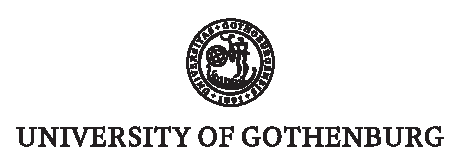
\includegraphics
{LO_GUeng_cenSV.eps} 
\end{center}
\endinput

%%% ACTA-frontmatter.tex
%%% Version 2021 (April)
%%% 
%%% COLOPHON
\newpage
\restoregeometry
%%% The following command redefines chapters to look like sections in the frontmatter.
\frontmatterchapters

%%% Failsafe
\fontsize{13}{18}\selectfont

\vspace*{\fill}

\begin{flushleft}
Thesis submitted for the Degree of Doctor of Philosophy in XX\\
Department of Philosophy, Linguistics and Theory of Science\\
University of Gothenburg
\end{flushleft}


\begin{flushleft}
\textcopyright\ 
\makeatletter{\MakeUppercase{\@author}}\makeatother, 20XX
\end{flushleft}

\begin{flushleft}
\makeatletter ISBN \@isbnp { (printed)}\makeatother\ (Contact ACTA via \url{acta@ub.gu.se})\\
\makeatletter ISBN \@isbnd { (pdf)}\makeatother\\
ISSN 0283-2380
\end{flushleft}

\begin{flushleft}
The publication is also available in fulltext at:

\url{http://XX}
\end{flushleft}

\begin{flushleft}
Subscriptions to the series and orders for individual copies sent to:\\
Acta Universitatis Gothoburgensis\\
PO Box 222, SE-405 30 G\"oteborg, Sweden \\
or to\\
\url{acta@ub.gu.se}
\end{flushleft}

\begin{flushleft}
Typeset in Adobe Garamond Pro, Arial, Garamond-Math,\\
Libertinus Sans, and Libertinus Mono using {\latexfont \XeLaTeX} and KOMA-Script
\end{flushleft}

\begin{flushleft}
Cover: 

XX (Write an explanatory note on the (possible) cover art, with page references to detailed information in the book.)
\end{flushleft}

\begin{flushleft}
Print:
XX, XX, 20XX
\end{flushleft}
% Failsafe
\fontsize{14}{18}\selectfont
 
 
%%% ABSTRACT

\chapter*{Abstract}
\fontsize{14}{18}\selectfont
\vspace{.5\baselineskip}

\setlength{\tabcolsep}{0pt} % to be restored later
\noindent\begin{tabular}{p{2.58cm}@{}ll}
\normalfont\fontsize{14}{18}\selectfont
%%% If your title is very long, and you have a subtitle, then use the eight lines below:
Title: & \makeatletter{\@title\ }\makeatother
\makeatletter
\ifx\@subtitle\@empty
\makeatother
\tabularnewline
\else
 -- \tabularnewline & \makeatletter{\@subtitle}\makeatother\tabularnewline
\fi

%%% If your title and subtitle are both very short, replace the eight lines above with the eight lines below.
%  Title: & \makeatletter\@title\ \makeatother
% \makeatletter
% \ifx\@subtitle\@empty
% \makeatother
% \tabularnewline
% \else
%  -- \makeatletter{\@subtitle}\makeatother\tabularnewline
% \fi

Author: & \makeatletter{\@author}\makeatother \\
    
Language: & English (with a summary in Swedish) \\

Department: & Philosophy, Linguistics and Theory of Science\\
 
Series: & \makeatletter{\@titlehead}\makeatother\\
 
ISBN: & \makeatletter{\@isbnp}\makeatother { (print)}\\
 
ISBN: & \makeatletter{\@isbnd}\makeatother { (digital)}\\
 
ISSN: & 0283-2380\\

Keywords: & XX \\
\end{tabular}
%%% Restoring tabcolsep to default.
\setlength{\tabcolsep}{6pt} 
\vspace{\baselineskip}

%%% Type your abstract below:
 
 \noindent XX.
 
 

 

%%% This is a reasonable place to add, e.g., a page for dedications, and such.
%%% For example using \chapter*{...}

\chapter*{Acknowledgements} 

XX

%%% Table of contents, with chapters, sections and subsections.
\setcounter{tocdepth}{2}

\addtocontents{toc}{\protect\thispagestyle{empty}} 
\tableofcontents

%%% If you dont have figures or tables, remove the following three lines of code.
%%% If you use both lists and they do not fit on the same page, replace the last line by
% \listoftables
\cleardoublepage 
\listoffigures
\bgroup\let\clearpage\relax\listoftables\egroup % This one!


%%% Set chapters to be formatted as chapters again.
%%% RB: Should not be placed elsewhere.
\mainmatterchapters
\endinput


%%% Shorten longest skips around math displays: was 14pt plus 3pt minus 7pt. The worst case 17pt is huge.
%%% Can be redefined if needed, but beware of resulting Bad Typography.
%%% Must be placed before mainmatter.
\setlength\abovedisplayskip{9pt plus 2pt minus 2pt}
\setlength\belowdisplayskip{9pt plus 2pt minus 2pt}
\setlength\belowdisplayshortskip{7pt plus 2pt minus 3pt} %default: 7 + 4 - 3

%%% The next line sets the page style to use the predefined headers.
%%% Must be placed before mainmatter.
\pagestyle{scrheadings}

%%% MAINMATTER
%%%
%%% Write your thesis, or include your chapter files below.
\mainmatter

\chapter{The very first chapter}
\lipsum[1]

\section{A section of the chapter}
\lipsum[2-3]

\subsection{With a subsection}
\lipsum[4]\footnote{A very short footnote.}

\subsubsection{A single subsubsection}
\lipsum[5]

\subsection{And another subsection}
\lipsum[6]

\section{The last section}
\lipsum[7-8]

\chapter{Another chapter}
\lipsum

\backmatter
%%% BACKMATTER
%%%
%%% This changes the name of the chapter Bibliography to References.
%%% Remove the following line for default name Bibliography.
\renewcommand{\bibname}{References}

%%% If that doesn't work, uncomment the line below. Unless you want
%%% your reference list to be called Bibliography.
% \renewcommand{\bibsection}{\chapter{\bibname}}

%%% To keep the bibliography non-empty. Should be removed once you've added your own references.
\nocite{test2021}

%%% I recommend using BibTeX. Replace the bibliography file with your own.
\bgroup
%%% ACTA formatting
\fontsize{12}{14}\selectfont
\bibliography{ACTA-template}
\egroup

%%% Alternatively, put your author-year-formatted \bibitems in here: 
% \begin{thebibliography}{99}
% \fontsize{12}{14}\selectfont
%
%%% If you're not using natbib, you might have to uncomment the following line to
%%% add the bibliography to the table of contents.
%% \addcontentsline{toc}{chapter}{\bibname}
% 
% \bibitem[Test, 2021]{test2021}
% Test, T. (2021).
% \newblock {\em {A Testing Publication}}.
% 
% \end{thebibliography}



 \chapter*{Sammanfattning}
%%% Add summary to table of contents, omitting any subsections.
%%% RB: Should not be placed elsewhere.
\selectlanguage{swedish}
\frenchspacing
\chaptermark{Sammanfattning}
\addcontentsline{toc}{chapter}{Sammanfattning på svenska}
\addtocontents{toc}{\protect\setcounter{tocdepth}{0}}
  %%% Add the Swedish summary of your thesis below.

\end{document}
